\documentclass[a4j,dvipdfmx]{jsarticle}
\usepackage{amsmath,amssymb}
\usepackage{siunitx}
\usepackage{bm}

\usepackage[margin=15truemm,nohead]{geometry}
\usepackage{qexam}

\usepackage{tikz}
\usetikzlibrary{calc}

\renewcommand{\div}{{\rm div}\hspace{1mm}}
\newcommand{\grad}{{\rm grad}\hspace{1mm}}
\newcommand{\rot}{{\rm rot}\hspace{1mm}}

\begin{document}
    \part*{理学同好会 ベクトル解析 テスト2}
    \question{問1}
        曲面の解析を行ってみる. 以下の問いに答えよ.
        \begin{qparts}
            \qpart 以下の曲面について, 適当なパラメータ表示を与えよ.ただし, \qref{q:球面のパラメータの問}については球面座標における$\phi,\theta$を用いよ.
            \begin{qlist}
                \qitem 球面$x^2+y^2+z^2=a^2$ \label{q:球面のパラメータの問}
                \qitem 半径$a$, 高さ$h$の円錐
                \qitem 曲面$z=f(x,y)$
                \qitem 1葉双曲面$\displaystyle \frac{x^2}{a^2}+\frac{y^2}{b^2}-\frac{z^2}{c^2}=1$
            \end{qlist}
            \qpart ここで, 曲面の基本的な量について, \qref{q:球面のパラメータの問}の球面を用いて復習しよう.ただし, 別のパラメータを$\phi,u$導入し, 通常の直角座標$(x,y,z)$との間に
            $x=u\cos\phi,y=u\sin\phi,z=\sqrt{a^2-u^2}$の関係があるとする.
            \begin{qlist}
                \qitem 曲面の第1基本量を求めよ.
                \qitem 球面上の微小面積$dS$を$d\phi,du$を用いて表せ.
                \qitem $dS$を曲面上の全域で積分して表面積を求め, $4\pi a^2$となることを確かめよ.
                \qitem 曲面の法線ベクトル$\bm{n}$を求めよ.
                \qitem 曲面の第2基本量を求めよ.
                \qitem 曲面のGauss曲率$K$と平均曲率$H$を求めよ.
            \end{qlist}
            \qpart 以下は簡単な証明問題である.
            \begin{qlist}
                \qitem 球の中心から放射状に生じた直線は常に球面と直交することを証明せよ.
                \qitem 曲面$\bm{r}(u,v)=[x(u,v),y(u,v),z(u,v)]$について, 曲面上の微小面積$dS$は以下の式で与えられることを示せ.ただし, $k$は定数.
                \begin{equation}
                    dS = \sqrt{\left(\frac{\partial(x,y)}{\partial(u,v)}\right)^2+\left(\frac{\partial(y,z)}{\partial(u,v)}\right)^2+\left(\frac{\partial(z,x)}{\partial(u,v)}\right)^2}dudv
                \end{equation}
                ここで$\displaystyle \frac{\partial(x,y)}{\partial(u,v)}$はヤコビアンである.
            \end{qlist}
            \qpart 以下の式で与えられる曲面について, Gauss曲率$K$が負の一定値を持つことを示せ.
                \begin{equation}
                    \bm{r}(u,v)=\left[k\sin u\cos v, k\sin u\sin v,k\left(\log\tan\frac{u}{2}+\cos v\right)\right]\quad (0<u<\pi,0\leq v\leq 2\pi)
                \end{equation}
                この曲面は,擬球と呼ばれる.擬球は負の一定曲率を持つが, $z=0$で尖点を持っている. 
        \end{qparts}
    \clearpage

    \question{問2}
        スカラー場・ベクトル場の各微分演算について考える. 以下の問いに答えよ.
        \begin{qparts}
            \qpart まずはベクトル場のイメージをつかもう. 次のベクトル場を図示せよ.
            \begin{qlist}
                \qitem $\bm{v}=[x^2,y^2]$
                \qitem $\bm{v}=[1,0]$
                \qitem $\bm{v}=[y,x]$
            \end{qlist}
            \qpart 次のスカラー場の勾配ベクトルを求めよ. ただし, $m,g,Q,\varepsilon_0$は定数とする.
            \begin{qlist}
                \qitem $U(x,y)=mgy$
                \qitem $U(x,y)=2x+y$
                \qitem $U(x,y,z)=mgy$
                \qitem $\displaystyle V(x,y,z)=\frac{Q}{4\pi\varepsilon_0\sqrt{x^2+y^2+z^2}}$
            \end{qlist}
            \qpart 次のベクトル場の発散, 回転を求めよ.
            \begin{qlist}
                \qitem $\bm{v}=[3,1,4]$
                \qitem $\bm{v}=[x^2,x,y]$
                \qitem $\displaystyle \bm{v}=\left[\frac{x}{\sqrt{x^2+y^2}},\frac{y}{\sqrt{x^2+y^2}}\right]$
            \end{qlist}
            \qpart 次の公式を証明せよ.
            \begin{qlist}
                \qitem $\div\grad f=\nabla^2f$
                \qitem $\rot\grad f = 0$
                \qitem $\div\rot \bm{v}=0$
                \qitem $\rot\rot\bm{v}=\grad\div\bm{v}-\nabla^2\bm{v}$
            \end{qlist}
        \end{qparts}
    \clearpage
    \question{問3}
        以下ではベクトル場上で積分を行う.
        \begin{qparts}
            \qpart まずは簡単な線積分で練習してみよう.以下の経路について, 線積分を実行せよ.ただし, $\bm{F}=[y^2,x+y^2]$とする.
            \begin{figure}[h]
                \centering
                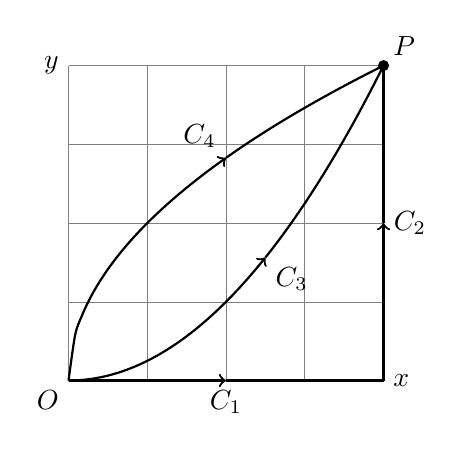
\begin{tikzpicture}
                    \draw [help lines] (0,0) grid (4,4);
                    \coordinate (O) at (0,0) node at (O) [below left] {$O$};
                    \coordinate (P) at (4,4) node at (P) [above right] {$P$};
                    \node at (4,0) [right] {$x$};
                    \node at (0,4) [left] {$y$};
                    
                    \fill (P) circle (2pt) ;

                    \draw[thick,->] (O) -- (2,0) node [below] {$C_1$};
                    \draw[thick] (2,0) -- (4,0);
                    \draw[thick,->] (4,0) -- (4,2) node [right] {$C_2$};
                    \draw[thick] (4,2) -- (4,4);

                    \draw[thick,domain=0:2.5,->] plot (\x,1/4*\x*\x) node [below right] {$C_3$};
                    \draw[thick,domain=2.5:4] plot (\x,1/4*\x*\x);

                    \draw[thick,domain=0:2,smooth,->] plot (\x,{2*sqrt(\x)}) node [above left] {$C_4$};
                    \draw[thick,domain=2:4,smooth] plot (\x,{2*sqrt(\x)});
                \end{tikzpicture}
                \caption{積分路}\label{積分路}
            \end{figure}
            \begin{qlist}
                \qitem 経路$C_1:0\leq x\leq 4,y=0$
                \qitem 経路$C_2:x=4,0\leq y\leq 4$
                \qitem 経路$C_1+C_2$
                \qitem 経路$C_3:\displaystyle y=\frac{1}{4}x^2\quad (0\leq x\leq 4)$
                \qitem 経路$C_4:\displaystyle y=2\sqrt{x} \quad (0\leq x\leq 4)$
            \end{qlist}
            また, $\bm{F}=[ax+by,bx+cy]\quad(q,b,c\text{は定数})$として, 上記の経路で同様に積分せよ.
        \qpart $C$を閉曲線とする. このとき以下の等式が成り立つことを示せ.
            \begin{equation*}
                \oint_C yzdx+zxdy+xydz = 0
            \end{equation*}
        \qpart $\Gamma$を原点を中心とする円とする. このとき以下の積分を求めよ.
            \begin{equation*}
                \oint_\Gamma \frac{x^3-3xy^2}{(x^2+y^2)^2}dx
            \end{equation*}
        \qpart 以下の面積分を計算せよ.ただし, 各$\bm{n}$は閉曲面$S$の外向きの単位法線ベクトル.
            \begin{qlist}
                \qitem $\bm{F}=[x^2,y^2,z^2]$で, $S$が原点中心で一辺の長さが2の立方体の表面のときの$\displaystyle \iint_S \bm{F}\cdot\bm{n}dS$
                \qitem $\bm{F}=\bm{r}$で, $S$が半径2, 高さ5の円柱面のときの$\displaystyle \iint_S\bm{F}\cdot\bm{n}dS$
                \qitem $S$を半径1の球表面とするときの, $\displaystyle\iint_S (x^4+y^4+z^4)dS$
            \end{qlist}
        \qpart 原点に置かれた質量$m$の質点から$r$離れた点にある単位質量の質点に働く力は
            \begin{equation}
                \bm{F}=-\frac{Gm}{r^3}\bm{r} \label{eq:万有引力の場}        
            \end{equation}
            である. ここで$G$は定数である. これは万有引力の場を表す.
            \begin{qlist}
                \qitem 働く力が式\eqref{eq:万有引力の場}と書ける理由を答えよ. (万有引力の大きさに関する式$F=G\frac{mM}{r^2}$から説明せよ.)
                \qitem 質点$m$を中心として半径$r$の球表面$S$を考える. $S$上で$\bm{F}$を積分して
                    \begin{equation*}
                        \iint_S \bm{F}\cdot d\bm{S} = -4\pi Gm
                    \end{equation*}
                    を示せ.
            \end{qlist}
        \qpart 最後に, 線積分を利用して閉曲線が原点をまわる回数を求めてみよう.次のベクトル場を考える.
            \begin{equation*}
                \bm{F}=\left[-\frac{y}{x^2+y^2},\frac{x}{x^2+y^2}\right]
            \end{equation*}
            以下の問いに答えよ.
            \begin{qlist}
                \qitem $\theta(x,y)=\arctan\left(\frac{y}{x}\right)$について, $\partial_x \theta,\partial_y \theta$を求めよ.
                \qitem 全微分$d\theta$を求めよ.
                \qitem $C$を任意の閉曲線として
                    \begin{equation}
                        \frac{1}{2\pi}\oint_{C} \bm{F}\cdot d\bm{r}
                    \end{equation}
                    が$C$が原点を回る回数であることを示せ.ただし, 反時計回りを正, 時計回りを負とする.
            \end{qlist}
        \end{qparts}
    \hrulefill  以上 \hrulefill

\end{document}